\newpage
\part{Functional requirement of the program}
\section{The project}
The goal of this project is to simulate the movement of a fluid through
different geometries. The program creates a box of a choosen size, builds a
geometry inside it and simulates the movement of a given fluid.
\section{Files}
In order to increase readability, the project is made of several files.
I made the choice to work with Object Oriented Programming.
\begin{itemize}
      \item main.py: This file calls for the needed functions/class
      \item matrices.py: This file contains the class ``Matrices'', it builds
            the geometry, the different matrices to plot and stores them
      \item plot.py: This file plots the matrices built in ``matrices.py''
      \item parameters.py: This file contains all the variables that can be 
          changed by the user
      \item data\_check.py: This file checks the variables and makes sure that
          the program will run
\end{itemize}

\section{Data}
This project uses several piece of data set by the user to work.
\begin{itemize}
      \item \py{Nx:} \textcolor{dtype}{\py{uint}} and
            \py{Ny:} \textcolor{dtype}{\py{uint}}, size of the domain
      \item \py{h:} \textcolor{dtype}{\py{uint}}, size of a cell
      \item \py{geometry: str}, choosen geometry
      \item \py{angle:} \textcolor{dtype}{uint}, angle of the
            widening/shrinkage geometry
      \item \py{vx: float}, initial fluid speed (Neuman's condition)
      \item \py{phi_ref: float}, reference velocity potential (Dirichlet's
            condition)
      \item \py{rho: float}, relative density of the fluid
      \item \py{pressure_init: float}, initial pressure of the fluid
\end{itemize}
Be careful in the case of a widening/shrinkage geometry!
In order for the program to generate a domain from one end to another, there is
a restriction on the angle, if the restriction is not met, the program will
output a ValueError. The restriction is as follows:
\[
      |angle| < \arctan{\left(\dfrac{0.5 \times N_y - 1}{N_x}\right)}
\]
The angle parameter should be set in degree, the program will convert it to
radians for the computation.

\section{Outputs}
As of the alpha version, the program outputs 4 pdf files, one for each plot.
The files are saved in a subfolder named \textbf{figures/} and the filenames
are set with the following rule:\\
\begin{center}
      \mintinline{python}{<data>_<geometry>_Nx=<Nx>_Ny=<Ny>.pdf}
\end{center}
\mintinline{python}{data} stands for the plotted data (potential, velocity,
streamlines, pressure).
\section{Concerning the running time}
Due to the function \py{numpy.linalg.solve()} being slow for
big matrices, the bigger the size of the domain, the higher the running time.\\
For a domain size of $\num{3600}$ cells ($\num{60} \times \num{60}$), it takes
around $\num{20}$ seconds to run, for a domain size of $\num{14400}$ cells
($\num{120} \times \num{120}$), it increases to $\num{23}$ minuts. 
\smallbreak{}
I searched for a faster method to solve the linear system in vain, thus I
recommend to stay on relatively low values for $N_x$ and $N_y$, the graphs are
easily readable for a value of $\num{60}$ each.
\smallbreak{}
By default, python only uses one CPU core when executing a program, the
solution to that problem is parallel programming, however I am not enough
experienced in that field to develop an optimized program.

\part{Internal structure of the program}
\section{Physical model}
In order to build the model, the program uses a squared structured meshe
model (matrix). The values are computed at each point of the matrix.

\subsection{Velocity potential field}
The velocity potential field is computed by solving a system of linear
equations. The result is computed using the matrix method, by solving the
equation $Ax = b$ we can find the potential flow value in each cell.\\
The matrix $A$, of size $N_\text{fluid} \times N_\text{fluid}$ stores 2
information per cell, the number of neighboring cells and the number of each
one of them. The number of neighbougring cells is stored in the diagonal of the
 matrix. Let $c$ be the number of a cell containing fluid and $n_c$ the number
 of neighbors for the cell $n$, the diagonal elements are defined as follows:
\[
      A_{n, n} = -n_c
\]
For each neighboring cell, some elements of the matrix are as follows:
\[
      A_{n, nb} = 1
\]
with $nb$ the number of a neighboring cell.\\

\section{Scientific computation algorithms}


\section{Constitutive elements}
\subsection{\py{main.py}}
This file is executable (without parameters input in the command).\\
After the imports, it will first call the file \py{check_data.py} to check the
type of the input data.\\
Then it will call the file \py{matrices.py} to initiate
the values of \py{G}, \py{M}, \py{cell_coords}, \py{A} and \py{b}.
\smallbreak{}
It then checks for the \py{recompute} value, if \py{True} or if there are no
existing \textbf{dat} files for the current parameters, it will call
the function \py{domain_check()} to display a warning if the domain is large.
It then calls the subroutine \py{make_data()} to compute \py{phi},
\py{grad_x}, \py{grad_y}, \py{grad_norm} and \py{pressure} and saves them in
\textbf{dat} files.\\
Else, it will use the existing dat files to generate the plots.
\smallbreak{}
Then it calls the function \py{load_data()} to read the \textbf{dat} files and
stores them in a dictionary and it initiate the file \py{plot.py} which will be
used to plot the different values.
\smallbreak{}
The last lines call the subroutine \py{plot_graphs} with different arguments
to plot and save all the wanted graphs.

\subsection{\py{data_check.py}}
This file has several subroutines and functions to rule the execution of the
program.

\subsubsection{\textcolor{func}{\py{data_check()}}}
The subroutine \textcolor{func}{\py{data_check()}} reads the value of each
parameter and checks that the type and the value are correct and will not cause
a crash of the program. If the value/type is incorrect, it will raise an error
and stop the program.

\subsubsection{\textcolor{func}{\py{existing_data()}}}
The function \textcolor{func}{\py{existing_data()}} will check for specific
files in the \textbf{dat/} subfolder. If at least one files is missing, it
returns \py{True} and the program will recompute all the data. Else it does
nothing.

\subsubsection{\textcolor{func}{\py{domain_check()}}}
The subroutine \textcolor{func}{\py{domain_check()}} is just a warning. It read the max value of
the matrix \py{M} plus one which is the number of fluid cells to compute.
If this number is higher than 5000, it will display a message warning the user
that the program can take some time to run. Then it asks if the user wants to
keep going. \py{"Yes"} will continue, \py{"No"} will stop the program and
anything other than that will stop the program aswell.

\subsection{\py{matrices.py}}
This class is where everything is computed, from start to end.

\subsubsection{\textcolor{func}{\py{__init__()}}}
\textcolor{func}{\py{__init__()}} stores the value of \py{G}, \py{M}, \py{cell_coords}, \py{b} and
\py{A} which will be used several times in the class.

\subsubsection{\textcolor{func}{\py{make_data()}}}
The subroutine \textcolor{func}{\py{make_data{}}} will call the functions that compute \py{phi},
\py{grax_x}, \py{grad_y}, \py{grad_norm} and \py{pressure}. Each function
will write the data in a \textbf{dat} file.

\subsubsection{\textcolor{func}{\py{load_data()}}}
The function \textcolor{func}{\py{load_data()}} reads the \textbf{dat} files and return the
values in a dictionary.

\subsubsection{\textcolor{func}{\py{build_g()}}}
The function \textcolor{func}{\py{build_g()}} takes 4 input arguments.
\begin{itemize}
      \item \py{Nx: int}
      \item \py{Ny: int}
      \item \py{geometry: str}
      \item \py{angle: int} of size 8 bits, in radians
\end{itemize}
It acts as a selector. Given a geometry, it will create a matrix \py{G} filled
with zeros and call the function \textcolor{func}{\py{build_geometry()}} with different input
values. There is no real point in this function in the alpha version since the
straight, widening and shrinkage geometries are generated from the same
function, with only the angle changing. However, it will prove useful in the
beta and gold version.

\subsubsection{\textcolor{func}{\py{build_geometry()}}}
The function \textcolor{func}{\py{build_geometry()}} takes 2 input arguments.
\begin{itemize}
      \item \py{G:} \textcolor{dtype}{\py{np.array}}
      \item \py{angle: int} of size 8 bits, in radians
\end{itemize}
The function returns the matrix \py{G}.\\
The function starts by computing \py{alpha} as the tangent of the angle.\\
It then uses it in a \py{for} loop to compute an offset which will be used to
build the geometry.\\
In case of a shrinkage geometry, the angle inputed is negative, the function
will flip horizontally the matrix. It then sets the inlet and outlet of the
domain.\\
Since the program will always compute \py{G} no matter what and to avoid some
problem, it will save the matrix only if \py{recompte == True}.

\subsubsection{\textcolor{func}{\py{build_index_matrices()}}}
The function \textcolor{func}{\py{build_index_matrices()}} takes 2 input arguments.
\begin{itemize}
      \item \py{Nx: int}
      \item \py{Ny: int} 
\end{itemize}
The function returns the matrix \py{M} and the array \py{cell_coords}.\\
It starts by creating the matrix \py{M} the shape of \py{G}, filled with zeros
and initiate a counter \py{count}. It then parses \py{M} and for each fluid
cell (\py{G[c, r] != 0}), it sets the value of \py{M[r, c]} to the value of the
counter and increment the counter by 1. All the other values are set to -1.\\
Then it create an array \py{cell_coords} of size \py{(M.max() + 1, 2)} and
sets the value of the counter back to zero. Then it parses the matrix \py{M}
and for each cell which value is not -1, it will store the coordinates of that
cell in the index \py{count} of the array \py{cell_coords} and increment the
counter.

\subsubsection{\textcolor{func}{\py{build_a()}}}
The function \textcolor{func}{\py{build_a()}} takes no input, it uses the imported data from
\py{parameters.py}.\\
The function returns the matrix \py{A}.\\
It starts by creating an array \py{A} of size
$(N_{\text{fluid}}, N_{\text{fluid}})$, filled with zeros. It then
parses the array \py{cell_coords} and for each inlet and fluid cell (the oulet
is not counted there), it counts the neighbors, stores their coordinates,
set the value of the diagonal depending on the neighbors and sets each
neighbor associated cell to 1. The diagonal cells corresponding to the outlet
are all set to 1.

\subsubsection{\textcolor{func}{\py{build_b()}}}
The function \textcolor{func}{\py{build_b()}} takes no input, it uses the
imported data from \py{parameters.py}.\\
It returns the array \py{b}.\\
It starts by creating an array \py{b} of size
\py{(cell_coords.shape[0], 1)}, filled with zeros.\\
It then parses the array. For each cell corresponding to the inlet, it sets the
value to \py{-vx * h} and for each value corresponding to the outlet, it sets
the value to \py{phi_ref}. The rest of the array is not modified.

\subsubsection{\textcolor{func}{\py{build_phi()}}}
The function \textcolor{func}{\py{build_phi()}} takes no input, it uses the
imported data from \py{parameters.py}.\\
This function is the slowest one since it compute the solution of $Ax = b$. For
that it uses the function \py{linalg.solve()} from \py{numpy}. Then it creates
an empty matrix \py{phi} and fills it with \py{numpy.nan}. It then parses
\py{x} and sets the value of each phi cell corresponding to the \py{x} value.
The other cells are not modified.\\
Finally, it saves the values in a \textbf{dat} file.

\subsubsection{\textcolor{func}{\py{build_gradient()}}}
The function \textcolor{func}{\py{build_gradient()}} takes no input, it uses the imported data
from \py{parameters.py}.\\
This function is rather big, but it is only a variation of the \py{gradient}
function from \py{numpy}. The function \py{numpy.gradient} does not work
the way I want with the \py{numpy.nan} values so I made my own.\\
It starts by loading the \textbf{dat} file containing the values of \py{phi}
and creates 2 empty matrices \py{grad_x} and \py{grad_y} the same shape as
\py{G} and fills them with \py{numpy.nan}. It the parse the \py{cell_coords}
array and sets the values of \py{grad_x} and \py{grad_y} following the centered
difference with step $2h$ mentioned in the scope statement. I then found that
the function \py{numpy.gradient} uses the same method. However, since the
borders of the matrix \py{phi} is filled with \py{numpy.nan} values, the
gradient is not computed at the outer edge of the domain.\\
To compute there values, I applied the impermeable wall condition specified in
the section \textbf{5.1} of the scope statement. We consider the 
\py{numpy.nan} cell with coordinates \py{[i - 1, j]} as a fictious cell with
the value of the cell \py{[i, j]}. This rule applies to the cells to the left
and to the right for \py{grad_x} and to the top and to the right for
\py{grad_y}.\\
It the computes the norm of the gradient (used later to plot the normalized
gradient).\\
Finally, it saves the 3 matrices in \textbf{dat} files.

\subsubsection{\textcolor{func}{\py{build_pressure()}}}
The function \py{build_pressure()} takes no input, it uses the imported data
from \py{parameters.py}.\\
The function starts by loading the \textbf{dat} files containing the values of
\py{grad_norm}.\\
It then creates an empty matrix \py{pressure} and fills it with \py{numpy.nan}.
Then, it computes the Bernoulli's constant $\mathcal{H}$ using the initial
values.\\
It then parses the array \py{cell_coords}, sets the inlet cells of the
\py{pressure} matrix to \py{pressure_init}, computes and sets the values for
each cell.\\
Finally, it saves the matrix in a \textbf{dat} file.

\subsection{\py{plot.py}}
The class is used to plot every piece of data.

\subsubsection{\textcolor{func}{\py{plot_graphs()}}}
The function \py{plot_graphs()} takes 2 input arguments.
\begin{itemize}
      \item \py{display: str}
      \item \py{data: dict}
\end{itemize}
This subroutine creates the figure, shows the matrix \py{G} (without
interpolation) and disables the axes as they are not needed in that kind of
plot. Then, depending on the \py{display} value, it will call other 
functions to plot the graphs and save them as \textbf{pdf} files.

\subsubsection{Data specific plotting functions}
Each one of the 4 next functions take 1 input argument.
\begin{itemize}
      \item \py{data: dict}
\end{itemize}
They return the plotted graph.\\
The 4 functions work the same way, they set the name of the graph and plot the
desired data.

\part{Quality approach}

\newpage
\part{Outcome examples}
\section{Input data}
The program needs some data to run. For the example, I found that a box of size
$\num{60} \times \num{60}$ is good enough. Obviously we can use a bigger box,
but the computing time increases exponentially as we increase the box size.
A smaller box can also produce acceptable results. I also choosed to use cells
of size 1 ($h = 1$). The geometry used is the \py{shrinkage} geometry.\\
Concerning the fluid, here are the data I choosed :
\begin{itemize}
      \item \py{rho} = 1, relative density of water
      \item \py{vx} = $\SI{1}{\meter\per\second}$, typical speed in a watering
            pipe
      \item \py{phi_ref} = 0
      \item \py{pressure_init} = $\SI{5}{\bar}$, typical pressure in a watering
            pipe
\end{itemize}

\section{Output}
\begin{figure}[htbp]
      \centering
      \begin{subfigure}{.45\textwidth}
            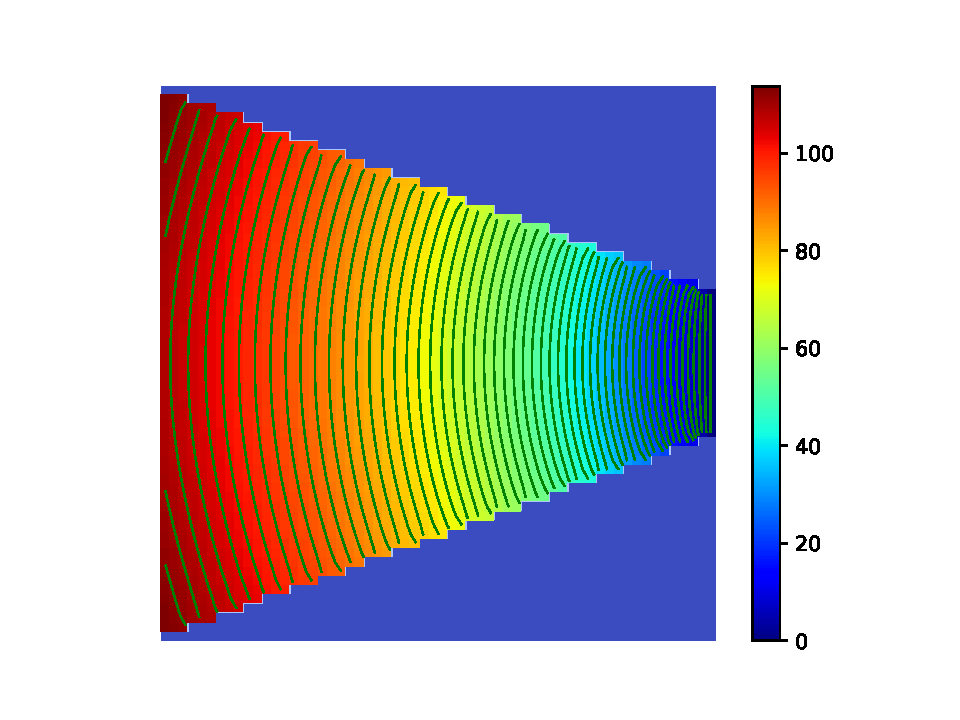
\includegraphics[width=.99\linewidth]{alpha_v2/figures/potential_shrinkage_Nx=60_Ny=60.pdf}
            \caption{Velocity potential field}\label{fig:vel_pot_field}
      \end{subfigure}
      \begin{subfigure}{.45\textwidth}
            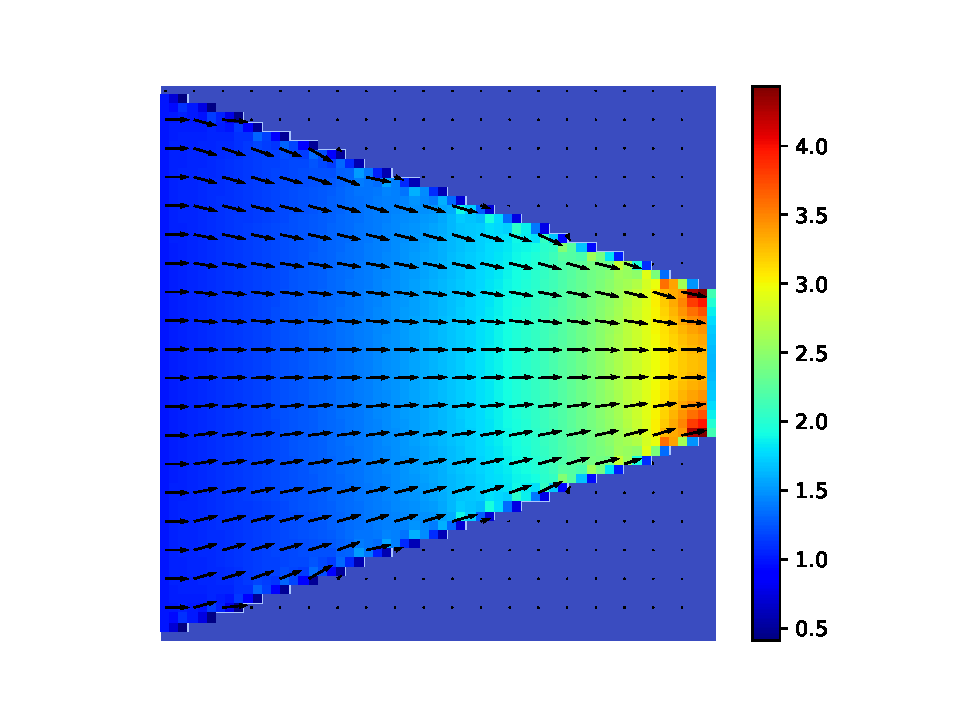
\includegraphics[width=.99\linewidth]{alpha_v2/figures/velocity_shrinkage_Nx=60_Ny=60.pdf}
            \caption{Velocity field}\label{fig:velocity_field}
      \end{subfigure}

      \centering
      \begin{subfigure}{.45\textwidth}
            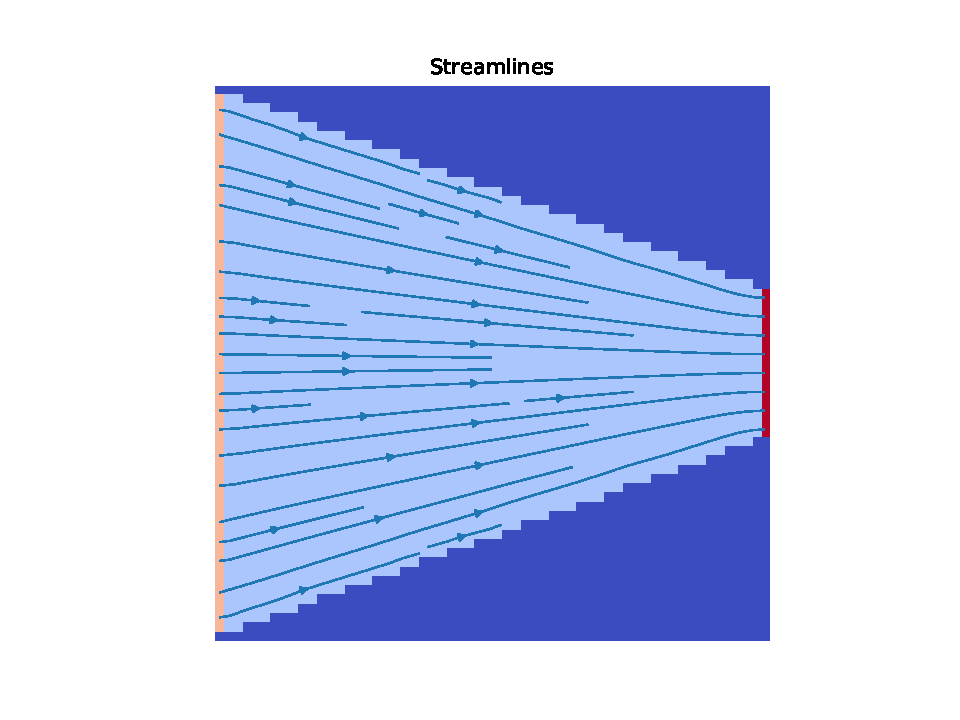
\includegraphics[width=.99\linewidth]{alpha_v2/figures/streamlines_shrinkage_Nx=60_Ny=60.pdf}
            \caption{Streamlines}\label{fig:streamlines}
      \end{subfigure}
      \begin{subfigure}{.45\textwidth}
            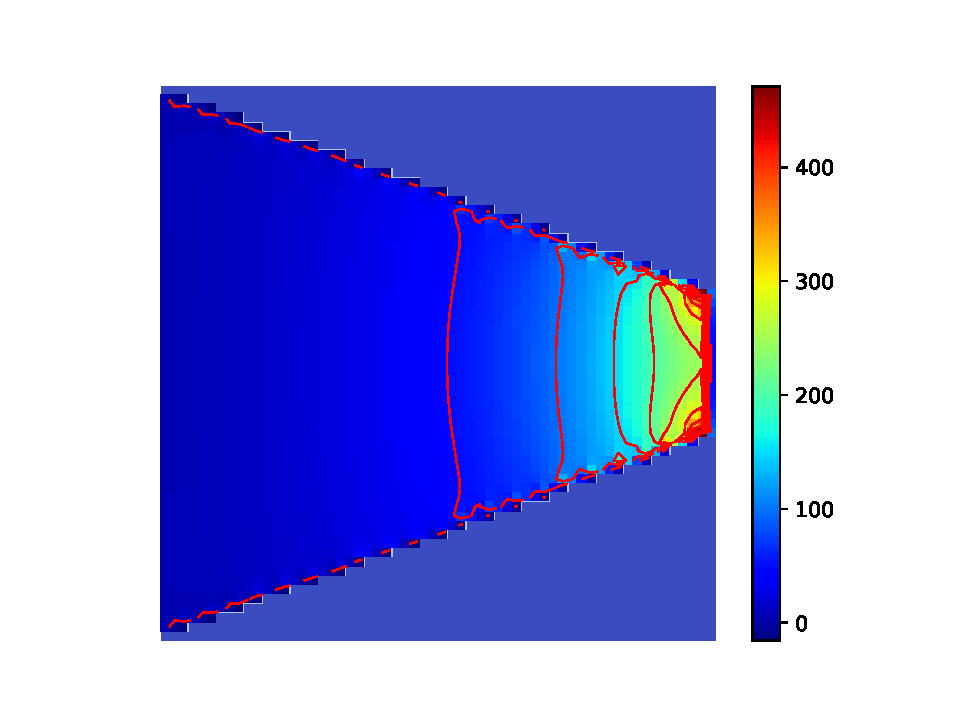
\includegraphics[width=.99\linewidth]{alpha_v2/figures/pressure_shrinkage_Nx=60_Ny=60.pdf}
            \caption{Pressure field}\label{fig:pressure_field}
      \end{subfigure}
      \caption{Results for \py{Nx} = \py{Ny} = \num{60} in a shrinkage geometry}
\end{figure}
\newpage
\section{Interpretation}
\subsection{Expectations}
The expected behavior for this kind of geometry (bottleneck) is that the fluid
(water in this case) will bump into the boundaries of the domain and converge
toward the center as it crosses the domain. Regarding the pressure of the
fluid, since the number of fluid particles is constant throughout the
simulation, we should observe a rise of pressure as the domain narrows.

\subsection{Observations}
Firstly, looking at \autoref{fig:velocity_field} and \autoref{fig:streamlines},
the water crosses the domain correctly and converges toward the center of the
domain. Despite some accuracy problems (the velocity in the edges seems off),
I can say that the simulation meets the expected behavior. It is mandatory to
normalize these vectors, else the output graph is not readable. However, the
bigger the domain, the bigger the number of vectors. As the size of the domain 
is $\num{60} \times \num{60}$, there are quite a lot of vectors to show. With
the default display, there are too much arrows on the graph and they are too
small to analyze anything, I added a small algorithm using interpolation to
reduce the number of arrows while keeping the data as accurate as possible.
Since the problem does not appear without the interpolation, I think it comes
from there. I will try to correct it in the beta. In the alpha version, the
streamlines are computed using the velocity, there should not be any problem
with them, they show the path of the fluid and it seems to be the right one.

\smallbreak{}
On the \autoref{fig:pressure_field}, it is clear that the pressure increases as
the fluid travels the domain. It is once again the expected behavior.



\newpage
\cite{potential-flow}
\newpage
\begin{multicols}{2}
    [\center{\printbibheading}]
    \printbibliography[heading=none]
\end{multicols}
